\documentclass[11pt]{article}
\input{/Users/markwang/.preamble}
\usepackage{stix}
\normalfont


\begin{document}

% arg1=pdfurl arg2=pagenum arg3=sectiontitle
\newcommand{\linksection}[3][../../bishop_pattern_recognition_and_machine_learning.pdf]{
    \subsection*{\href[page=#2]{#1}{#3}}
}

\newcommand{\linkinline}[3][../../bishop_pattern_recognition_and_machine_learning.pdf]{
    \noindent\href[page=#2]{#1}{#3}
}

\renewcommand{\norm}[1]{\left\lVert#1\right\rVert}
\renewcommand{\E}[2][]{\mathbb{E}_{#1}\left\{#2\right\}}
\newcommand{\var}[1]{var\{#1\}}
\newcommand{\cov}[1]{cov\{#1\}} 
\newcommand{\normal}[1]{\mathcal{N}\left(#1\right)}
\newcommand{\exponents}[1]{exp\left\{#1\right\}}

\newcommand{\bmu}{\boldsymbol{\mu}}
\newcommand{\bpi}{\boldsymbol{\pi}}
\newcommand{\bTheta}{\boldsymbol{\Theta}}
\newcommand{\bSigma}{\boldsymbol{\Sigma}}
\newcommand{\bphi}{\boldsymbol{\phi}}

\newcommand{\calL}{\mathcal{L}}
\newcommand{\calE}{\mathcal{E}}
\newcommand{\calR}{\mathcal{R}}
\newcommand{\calC}{\mathcal{C}}
\newcommand{\calD}{\mathcal{D}}
\newcommand{\bx}{\matr{x}}
\newcommand{\bt}{\matr{t}}
\newcommand{\bw}{\matr{w}}
\newcommand{\bX}{\matr{X}}
\newcommand{\bZ}{\matr{Z}}
\newcommand{\bz}{\matr{z}}
\newcommand{\bu}{\matr{u}}



\newcommand{\lebpar}[2]{\frac{\partial #1}{\partial #2}}
\newcommand{\qqqquad}{\quad \quad \quad \quad}

\newcommand{\condi}[3]{#1 \Vbar #2 \,|\, #3}
\newcommand{\notcondi}[3]{#1 \not\Vbar #2 \,|\, #3}

\linksection{375}{8 Graphical Models}
\linksection{376}{8.1 Bayesian Networks}

\begin{defn*}
    \textbf{Concepts}
    \begin{enumerate}
        \item \textbf{Graphical Model} The joint distribution defined by the graph is given by the product, over all nodes of the graph, of a conditional distribution for each node conditioned on the variable corresponding to the parents of that node in the graph
        \[
            p(\mathbf{x}) = \prod_{k=1}^K p(x_k | parent(x_k))
        \]
        which represents \textbf{factorization properties} of the joint distribution for a directed graphical model
        \begin{enumerate}
            \item \textbf{Node} 
            \begin{enumerate}
                \item \textbf{Open Circle} Random variable 
                \begin{enumerate}
                    \item \textbf{Shaded} Observed variable, i.e. variable $\{t_n\}$ from the training set, for setting the variable to some observed value
                    \item \textbf{Unshaded} Latent variable
                \end{enumerate}
                \item \textbf{Solid Circle (Dot)} Deterministic parameter 
            \end{enumerate}
            \item \textbf{Link} probabilistic relationships between these variables
            \item \textbf{Plate} labelled with $N$ indicate $N$ nodes of a certain kind by drawing a single representative node and surround it with a box
        \end{enumerate}
        \item \textbf{Bayesian Polynomial Regression}
        \begin{enumerate}
            \item \textbf{Joint Distribution}
            \[
                p(\bt,\bw) = p(\bw) \prod_{n=1}^N p(t_n | \bw)
                \qquad 
                p(\bt,\bw| \bx, \alpha, \sigma^2) = p(\bw|\alpha) \prod_{n=1}^N p(t_n |\bw, x_n, \sigma^2)
            \]
            \item \textbf{Posterior distribution}
            \item \textbf{Predictive distribution}
        \end{enumerate}
        \item \textbf{Generative Models}
        \item \textbf{Discrete Variable}
    \end{enumerate}
\end{defn*}

\linksection{388}{8.2 Conditional Independence}


\begin{defn*}
    \textbf{Conditional Independence}
    \begin{enumerate}
        \item \textbf{Goal} Infer conditional indepedence from graph structure 
        \item \textbf{Conditional Independence} $a$ is conditionally independent of $b$ given $c$, denoted as $\condi{a}{b}{c}$, if either is true 
        \[
            p(a|b,c) = p(a|c)
            \qquad \text{or} \qquad 
            p(a,b|c) = p(a|b,c)p(b|c) = p(a|c)p(b|c)
        \]
        in other words, joint distribution of $a$ and $b$ factorizes into product of marginal distribution of $a$ and marginal distribution of $b$ 
    \end{enumerate}
\end{defn*}

\begin{defn*}
    \textbf{3 examples}
    \begin{enumerate}
        \item For \textbf{tail-to-tail} node $c$, presence of path connecting $a$ and $b$ via a tail-to-tail node causes $a,b$ be dependent, however the conditioned node 'blocks' the path from $a$ to $b$ and causes $a$ and $b$ to become conditionally independent
        \begin{center}
            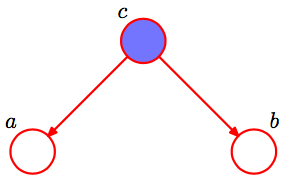
\includegraphics[width=5cm]{example1.png}
        \end{center}
        Joint distribution can be derived from the graph 
        \[
            p(a,b,c) = p(a|c)p(b|c)p(c)
        \]
        Note $\notcondi{a}{b}{\emptyset}$ ($a,b$ are dependent) when $c$ not observed
        \[
            p(a,b) = \sum_c p(a,b,c) = \sum_c p(a|c)p(b|c)p(c) 
            \overset{normally}{\neq} p(a)p(b)
        \]
        But $\condi{a}{b}{c}$ ($a,b$ are conditionally independent) when $c$ is observed (conditioned)
        \[
            p(a,b|c) = \frac{p(a,b,c)}{p(c)} = p(a|c)p(b|c)
        \]
        \item For \textbf{head-to-tail} node $c$, presence of path connecting $a$ and $b$ causes $a,b$ to be dependent. If we observe $c$, this observation blocks the path from $a$ to $b$ so we obtain conditional independence 
        \begin{center}
            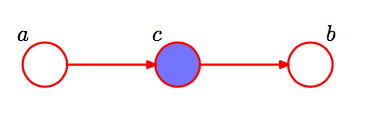
\includegraphics[width=5cm]{example2.png}
        \end{center}
        Joint distribution can be derived from the graph 
        \[
            p(a,b,c) = p(a)p(c|a)p(b|c)
        \]
        Note $\notcondi{a}{b}{\emptyset}$ ($a,b$ are dependent) when $c$ not observed
        \[
            p(a,b) = \sum_c p(a,b,c) = p(a) \sum_c p(c|a)p(b|c) = p(a)p(b|a)
            \overset{normally}{\neq} p(a)p(b)
        \]
        But $\condi{a}{b}{c}$ ($a,b$ are conditionally independent) when $c$ is observed (conditioned)
        \[
            p(a,b|c) = \frac{p(a,b,c)}{p(c)} = \frac{p(a)p(c|a)}{p(c)} p(b|c) \overset{bayes}{=} p(a|c) p(b|c)
        \]
        \item For \textbf{head-to-head} node $c$. When $c$ is unobserved, it blocks the path, and $a,b$ independent. However conditioning on $c$ unblocks the path and renders $a,b$ dependent. In general, a head-to-head path will become unblocked if either the node, or any of its descendents, is \textbf{observed}
        \begin{center}
            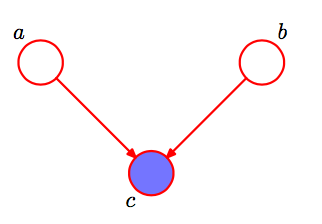
\includegraphics[width=5cm]{example3.png}
        \end{center}
        Joint distribution can be derived from the graph 
        \[
            p(a,b,c) = p(a)p(b)p(c|a,b)
        \]
        Note $\condi{a}{b}{\emptyset}$ ($a,b$ are independent) when $c$ not observed
        \[
            p(a,b) = \sum_c p(a,b,c) = p(a) p(b) \sum_c p(c|a,b) = p(a)p(b)
        \]
        But $\notcondi{a}{b}{c}$ ($a,b$ are conditionally dependent) when $c$ is observed (conditioned)
        \[
            p(a,b|c) = \frac{p(a,b,c)}{p(c)} = \frac{p(a)p(b)p(c|a,b)}{p(c)} \overset{normally}{\neq} p(a|c) p(b|c)
        \]
    \end{enumerate}
    \item \textbf{Summary} tail-to-tail or head-to-tail node leaves path unblocked unless it is observed in which case it blocks the path. By contrast, head-to-head node blocks a path if it is unobserved, but once the node, and/or at least one of its descendents, is observed the path becomes unblocked
\end{defn*}
 


 
\begin{defn*}
    \textbf{d-separation property} For directed graphs, where $A,B,C$ are nonintersecting sets of nodes. We want to know if $\condi{A}{B}{C}$ is implied by the graphical model. We consider \textbf{all paths} from any node in $A$ to any node in $B$. A path is \textbf{blocked} if it includes either 
    \begin{enumerate}
        \item \textbf{head-to-tail} or \textbf{tail-to-tail} node in set $C$ (observed)
        \item \textbf{head-to-head} node and all of its descendent are not in set $C$ (not observed)
    \end{enumerate}
    If all paths are blocked, then $A$ is said to be d-separate from $B$ by $C$, and the joint distribution over all variables in the graph satisfies $\condi{A}{B}{C}$. We consider parameters of model as behaving in the same way as observed nodes, but they do not have parents, so all paths through these nodes will be tail-to-tail and hence blocked, so play no role in d-separation
\end{defn*}

\begin{defn*}
    \textbf{Markov Blanket} (\linkinline{398}{derivation}) of a node $\bx_i$ is the set of nodes comprising the parents, the children and the co-parents. It has the property that the conditional distribution of $\bx_i$ conditioned on all the remaining variables in the graph, is dependent only on the variables in the Markov blanket. 
    \[
        p(\bx_i | \bx_{j\neq i})
        = \frac{p(\bx_1, \cdots, \bx_D)}{\sum_{\bx_i} p(\bx_1, \cdots, \bx_D)}
        = \frac{\prod_k p(\bx_k | parent(\bx_k))}{\sum_{\bx_i} \prod_k p(\bx_k | parent(\bx_k))}
    \]
    where terms $p(\bx_k|parent(\bx_k))$ that doesnt involve $\bx_i$ directly in the summation can be factored out and canceled with numerator. The terms that cannot be factored are either $p(\bx_i | parent(\bx_i))$ and $p(\bx_k|parent(\bx_k))$ where $\bx_i \in parent(\bx_k)$ Equivalently, the conditional distribution $\bx_i$ conditioned on its non-descendents is dependent only on $parent(\bx_i)$
    \begin{center}
        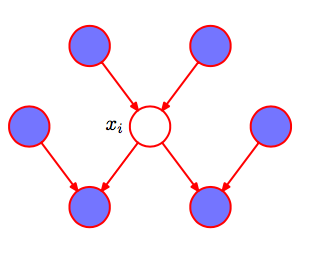
\includegraphics[width=5cm]{markov_blanket.png}
    \end{center}
\end{defn*}


 


\end{document}
